% DO NOT COMPILE THIS FILE DIRECTLY!
% This is included by the other .tex files.

\begin{frame}[t,plain]
\titlepage
\end{frame}

\begin{frame}[t]{Context}
\begin{itemize}
\item Many problems have the following structure:
  \begin{itemize}
  \item There are $N$ objects in a region, and we don't know the value of $N$
  \item Each object has properties $\mathbf{x}_i$
  \item We have some data $\mathcal{D}$ which we want to use to infer both $N$
        and $\{\mathbf{x}_i\}$.
  \end{itemize}
\end{itemize}
\end{frame}

\begin{frame}[t]{Motivating Problem I}
\begin{itemize}
\item How many sinusoids are in this data?
\end{itemize}
\begin{center}
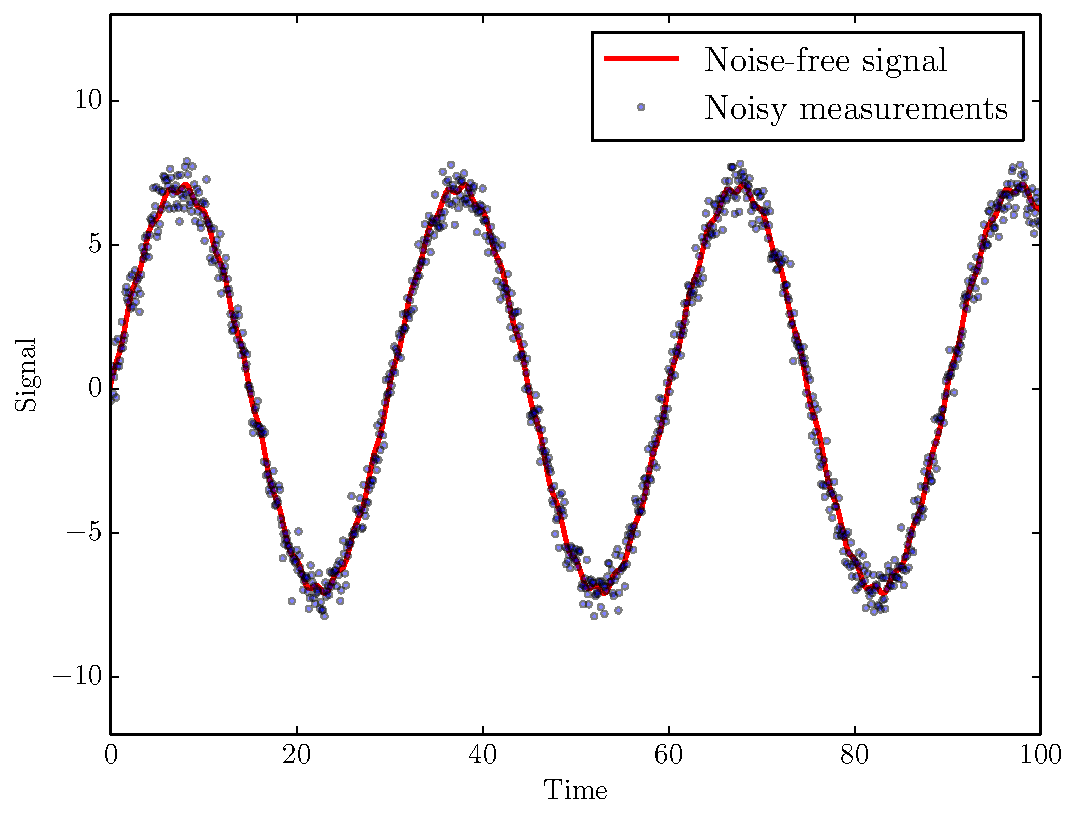
\includegraphics[scale=0.35]{sinewave_data.pdf}
\end{center}
\begin{itemize}
\item Also, what are their periods, amplitudes and phases?
\end{itemize}
\end{frame}

\begin{frame}[t]{Motivating Problem II}
\begin{itemize}
\item How many sinusoids are in this data?
\end{itemize}
\begin{center}
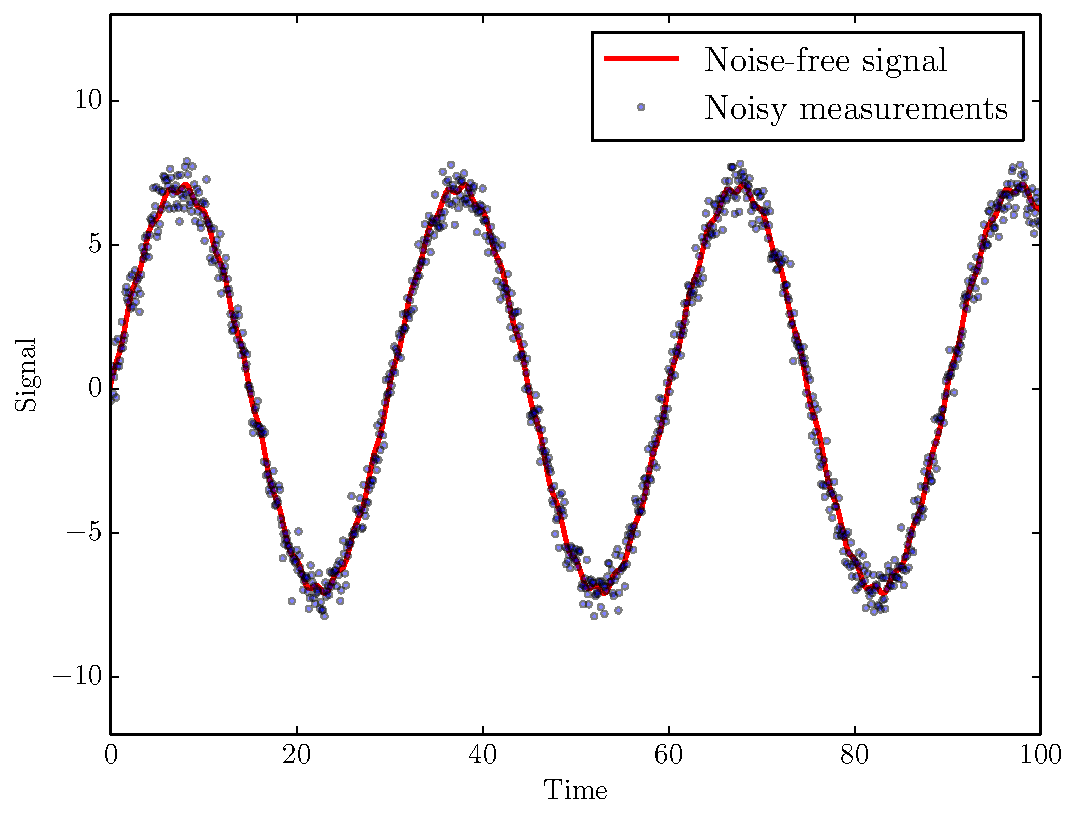
\includegraphics[scale=0.35]{sinewave_data.pdf}
\end{center}
\begin{itemize}
\item Also, what are their periods, amplitudes and phases?
\end{itemize}
\end{frame}

